 \documentclass[10pt, letterpaper]{article}
\usepackage[top=80pt,bottom=80pt,left=60pt,right=60pt]{geometry}
\usepackage{tabularx}
\usepackage{float}
\usepackage{titling}
\newcommand{\subtitle}[1]{%
  \posttitle{%
    \par\end{center}
    \begin{center}\large#1\end{center}
    \vskip0.5em}%
}
\usepackage{pgfplotstable}
\usepackage{tikz}
\usepackage[section]{placeins}
\usepackage[utf8]{inputenc}
\usepackage{csvsimple}
\usepackage{subfig}

\begin{document}

  \title{Internal Assessment: The Impact of the Sphere's Radius on the Sphere's Angular Velocity}
  \subtitle {IB Physics II Period 6, Dr. Petach}
  \date{19 October 2015}
  \author{Jackson Chen}
  \maketitle

  \section{Design}

    \subsection{Research}

    The aim of the experiment is to investigate the relationship between radius and
    angular velocity for the linear motion of a sphere unraveling from a string at a
    fixed height. This will be done by changing the radius of the sphere that is being
    dropped through the use of various sizes balls that are unraveled from the string
    and then measuring the linear velocity of the falling ball using a photogate.
    The purpose of the string is to cause the ball to rotate while falling, due to the
    nature of its unraveling motion.

    Prior to the experiment, I derived a relationship between the radius and the angular
    velocity of the rotational motion of the falling ball by the force analysis of the
    airplane, the definition of a period, and the radius of the flight path. Section \ref{sssec:derivation}
    will more specifically detail the derivation. The derived relationship predicted
    that period and height will follow an inverse relationship. The experiment itself
    was to test if Newtonian physics upheld this inverse relationship with tangible experimentation.

    \subsection{Variables}
    The independent variable is the radius of the sphere. The dependent variable is the
    angular velocity of the ball as it passes through the photogate. The controlled variables
    include the height of the initial position of the ball that is attached to the clamp,
    material of the string, the photogate, and the properties of the surrounding environment.

    \subsection{Apparatus}
    \begin{itemize}
      \item Photogate
      \item Four different sizes balls that are relatively uniform spheres
      \item String
      \item DataWorks software that reads data from the photogate
      \item Ring stand with clamp
      \item Meter stick
    \end{itemize}

    \subsection{Procedure}
    \begin{enumerate}
      \item Attach a clamp to a ringstand
      \item Place a photogate toward the bottom of the ringstand so that the ball will drop through it.
      \item Connect the photogate to the DataWorks software, such that it reads the linear velocity of the falling ball
      \item Measure the height difference between the placement of the clamp and the photogate along the ring stand using a meter stick
      \item Pick a ball, measure it radius using a meter stick
      \item Tie one end of the string to a clamp attached to a ring stand, and the other end around the ball
      \item Carefully wrap the string around the ball until the ball is level with the clamp
      \item Drop the ball so that it falls through the photogate
      \item Record the linear velocity that is measured by the photogate
      \item Repeat steps 6 to 9 for six trials
      \item Repeat steps 5 through 10 for the four different balls
    \end{enumerate}

    \subsection{Diagram}
    \begin{figure}[!htb]
      \centering
      \parbox{2.75in} {
        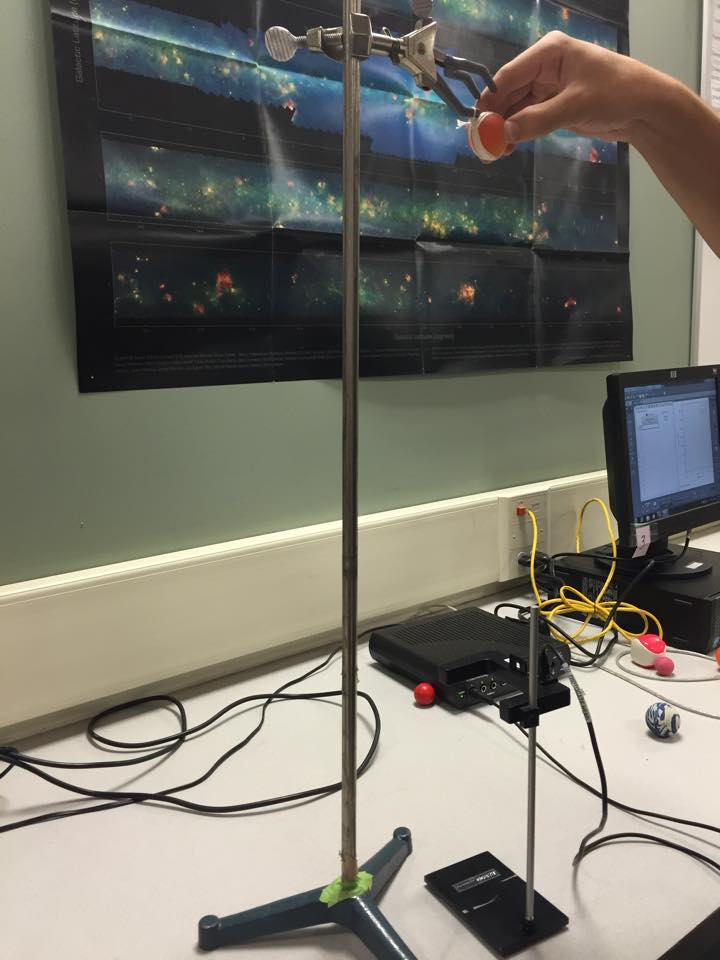
\includegraphics[scale=0.233]{img/setup.jpg}
        \caption{Picture of the experiment setup}
      }
      \begin{minipage}{2.75in}
        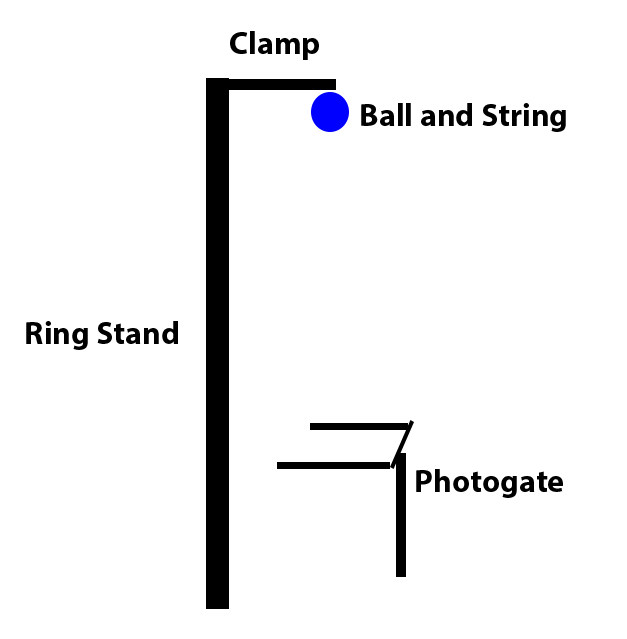
\includegraphics[scale=0.7]{img/apparatus.png}
        \caption{Diagram of the experiment setup}
      \end{minipage}
    \end{figure}

  \section{Data}

    \subsection{Data Collection}
      \begin{table}[H]
      \centering
      \pgfplotstabletypeset[
          col sep=comma,
          string type,
          header=true,
          every head row/.style={before row=\hline, after row=\hline},
          every last row/.style={after row=\hline}
          ]{data/hackeysack.csv}
      \caption{Data for six trials with ball radius of 2.34 cm.}
      \end{table}

      \begin{table}[H]
      \centering
      \pgfplotstabletypeset[
          col sep=comma,
          string type,
          header=true,
          every head row/.style={before row=\hline, after row=\hline},
          every last row/.style={after row=\hline}
          ]{data/bigball.csv}
      \caption{Data for six trials with ball radius of 1.90 cm.}
      \end{table}

      \begin{table}[H]
      \centering
      \pgfplotstabletypeset[
          col sep=comma,
          string type,
          header=true,
          every head row/.style={before row=\hline, after row=\hline},
          every last row/.style={after row=\hline}
          ]{data/mediumball.csv}
      \caption{Data for six trials with ball radius of 1.69 cm.}
      \end{table}

      \begin{table}[H]
      \centering
      \pgfplotstabletypeset[
          col sep=comma,
          string type,
          header=true,
          every head row/.style={before row=\hline, after row=\hline},
          every last row/.style={after row=\hline}
          ]{data/smallball.csv}
      \caption{Data for six trials with ball radius of 1.40 cm.}
      \end{table}
    \subsection{Data Processing}

    \subsubsection{Deriving the relationship between radius and angular velocity} \label{sssec:derivation}

  \section{Conclusion}

    \subsection{Evaluation}

    \subsection{Improvements}

\end{document}
